% This is where Assessors will be looking for signs of success and for evidence of thorough and systematic 
% evaluation as discussed in Section 8.3. Sample output, tables of timings and photographs of workstation screens,
% oscilloscope traces or circuit boards may be included. A graph that does not indicate confidence intervals will 
% generally leave a professional scientist with a negative impression.

% As with code, voluminous examples of sample output are usually best left to appendices or omitted altogether.
% There are some obvious questions which this chapter will address. How many of the original goals were achieved? 
% Were they proved to have been achieved? Did the program, hardware, or theory really work?
% Assessors are well aware that large programs will very likely include some residual bugs. It should always be 
% possible to demonstrate that a program works in simple cases and it is instructive to demonstrate how close it 
% is to working in a really ambitious case.

% ~2000 words

\documentclass[final,dissertation.tex]{subfiles}
\begin{document}

\chapter{Evaluation} \label{chapter:evaluation}

In this chapter, I evaluate my project in context of the project's success criteria. Namely, I will show that my library is binary compatible with the existing Python library, and various metrics such as bandwidth and latency overheads are graphed. Analysis of the viability of Loopix on mobile devices is also presented.

\section{Functional Testing}

Key functionality of the Loopix client library is the ability to connect to a Loopix network consisting of nodes running the original Python code. This is tested in two ways: unit tests and integration tests.

\textbf{Unit tests.} The Java Sphinx library uses the JUnit unit testing library. Output of the various keyed hash functions, key derivation functions, and LIONESS encryption and decryption is compared between the Java and Python implementations. Output from the creation of Sphinx packets is also compared. Random functions had to be stubbed out, as random padding and keys are generated and would prevent a byte-for-byte comparison between implementations. The Java test suite also attempts to decode Sphinx packets generated by the Python code. The same methodology is applied to the Loopix library. The results show that my library is able to generate the same bitstrings as the Python code, and it is able to decode packets generated by the Python code.

\textbf{Integration tests.} A test network is initially setup with entirely Python clients, providers and mix nodes. To test that the Java client is functional and compatible with the Python nodes, some of the Python clients are replaced with Java clients. Network behaviour is then observed to ensure correctness. An example of an issue found in early testing is the usage of incorrect time units when generating delays. The Java code was producing packets with delays in milliseconds, which were then intepreted as seconds by the Python nodes. This resulting in Python nodes delaying packets $1000x$ longer than expected.

\section{Performance}

\subsection{Experimental Setup}

All experiments were run on the Amazon EC2 platform, on a single \verb|m5.12xlarge| instance running 16.04 Ubuntu with 48 virtual cores on a 2.5 GHz Intel Xeon Scalable processor with 192GB of RAM. Every experiment was run with a network topology of 4 providers and 3 layers of mix nodes with 2 mix nodes in each layer for a total of 6 mix nodes. The number of clients and network parameters are varied accordingly for each experiment. Experiments were run for 3.5 minutes, with data collected after 30 seconds had passed to allow the network to initialise. Hardware limitations such as limited storage prevented longer running experiments.

\subsection{Bandwidth}
 
The bandwidth overhead of Loopix is evaluated by measuring the rate of outgoing messages, cover and real, against an increasing overall rate at which nodes send messages. Incoming messages are not measured, as it is fixed and predictable for clients. To measure bandwidth, packet traces were captured using \verb|tcpdump|. Static private keys allowed the decryption of captured packets to determine the type of message. Values were averaged over 3 repetitions and the error bars are the standard deviation.

Each packet has a fixed size of 2079 bytes, with a Sphinx header and body size of 1024 bytes each. The size parameter can be tuned for specific applications, and as such results presented in this section are in terms of messages rather than bytes.

The delay parameter \verb|EXP_PARAMS_DELAY| is set to 0.001 ($\mu = 1000$) such that the average delay per hop is \SI{1}{\milli\second}. There are 100 Java clients and 100 Python clients sending messages at rate $\lambda$ each. $\lambda$ is the sum of real, loop, and drop rates where $\text{Pois}(\lambda) = \text{Pois}(\lambda_R) + \text{Pois}(\lambda_L) + \text{Pois}(\lambda_D)$. The experiment was performed with parameters $\lambda_R = \lambda_L = \lambda_D = 0.1$ messages per second for a single client, increasing by $0.1$ messages per second each iteration such that $\lambda_R = \lambda_L = \lambda_D = \{0.1, 0.2, ..., 2.9, 3.0\}, \lambda = \{0.3, 0.6, ..., 8.7, 9.0\}$. Mix nodes also send loop messages at rate $\lambda_L$.

\begin{figure}[h]
	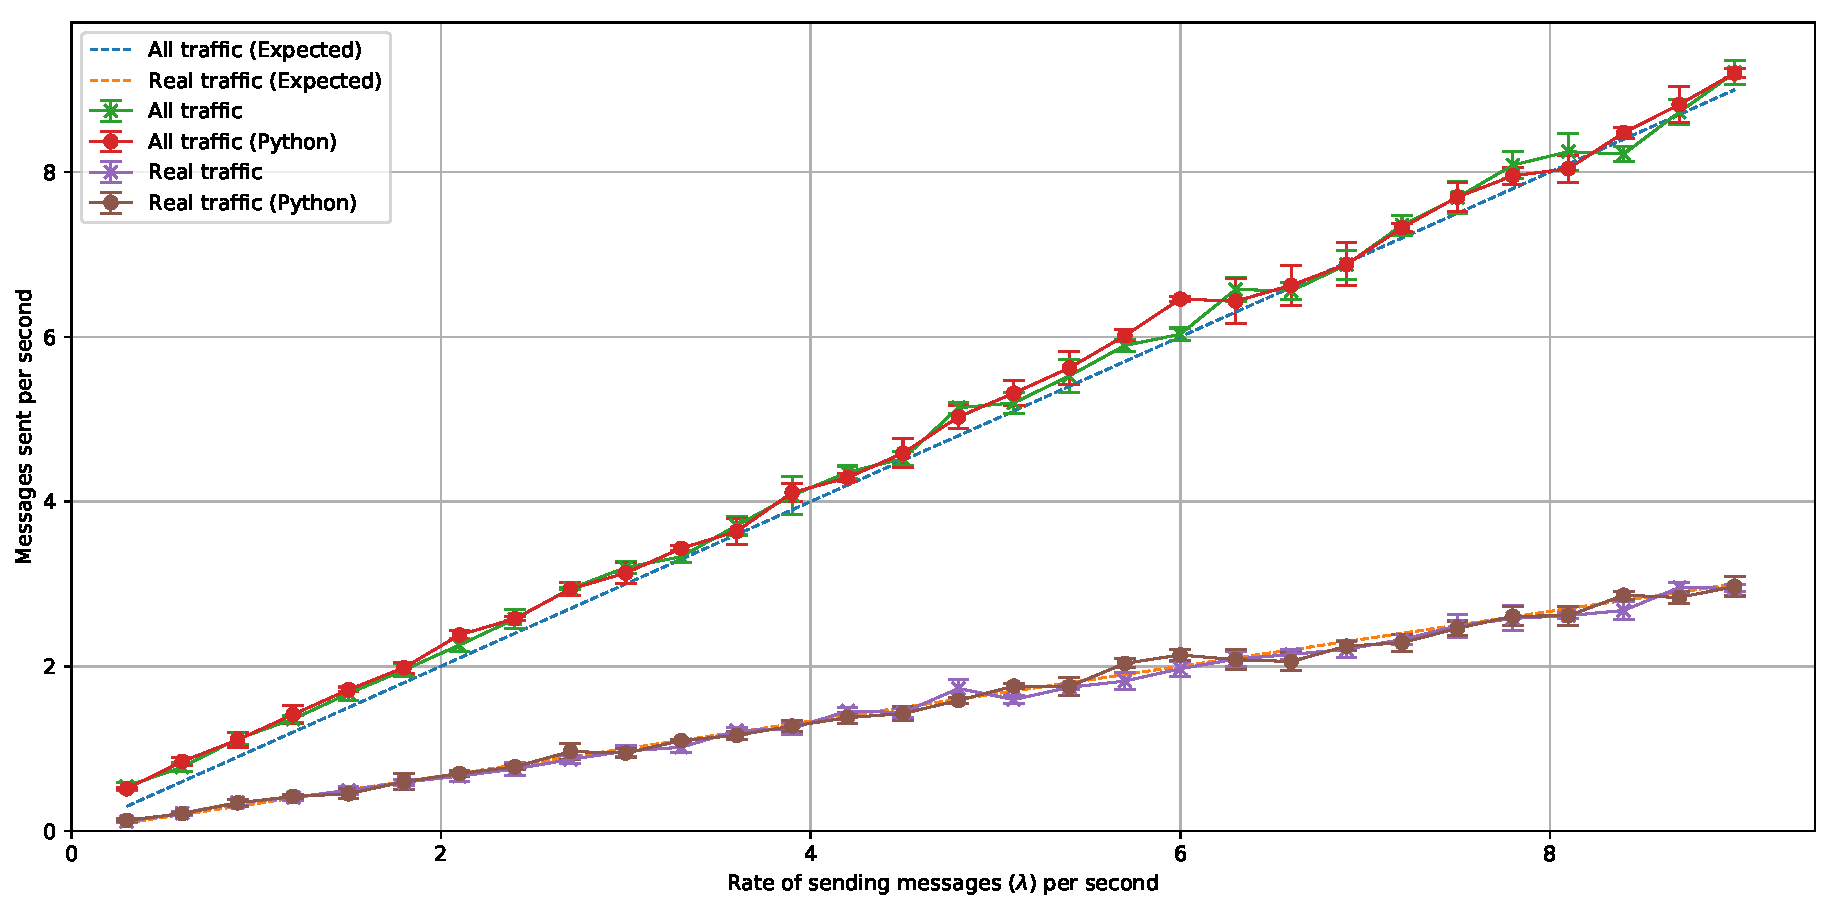
\includegraphics[width=\linewidth]{../figs/client_bandwidth}
	\caption{Overall sent traffic and real traffic per second for a single Java and Python client.}
	\label{fig:client_bandwidth}
\end{figure}

Figure~\ref{fig:client_bandwidth} shows the sending rate of all traffic and rate of real traffic of both the Java and Python client versus the overall sending rate $\lambda$ of a client. Observe that the Java client performs similarly to the Python client, and falls within the expected average rates predicted by a Poisson process. This is evidence that my implementation behaves similarly to the Python implementation and there are no obvious issues.

It is important to note that the $\lambda_R$ parameter determines the amount of real traffic in the network. Thus the parameter can be adjusted by a client depending on the amount of traffic in the network, with a potential loss of anonymity if there is insufficient cover traffic in the network.

\begin{figure}[h]
	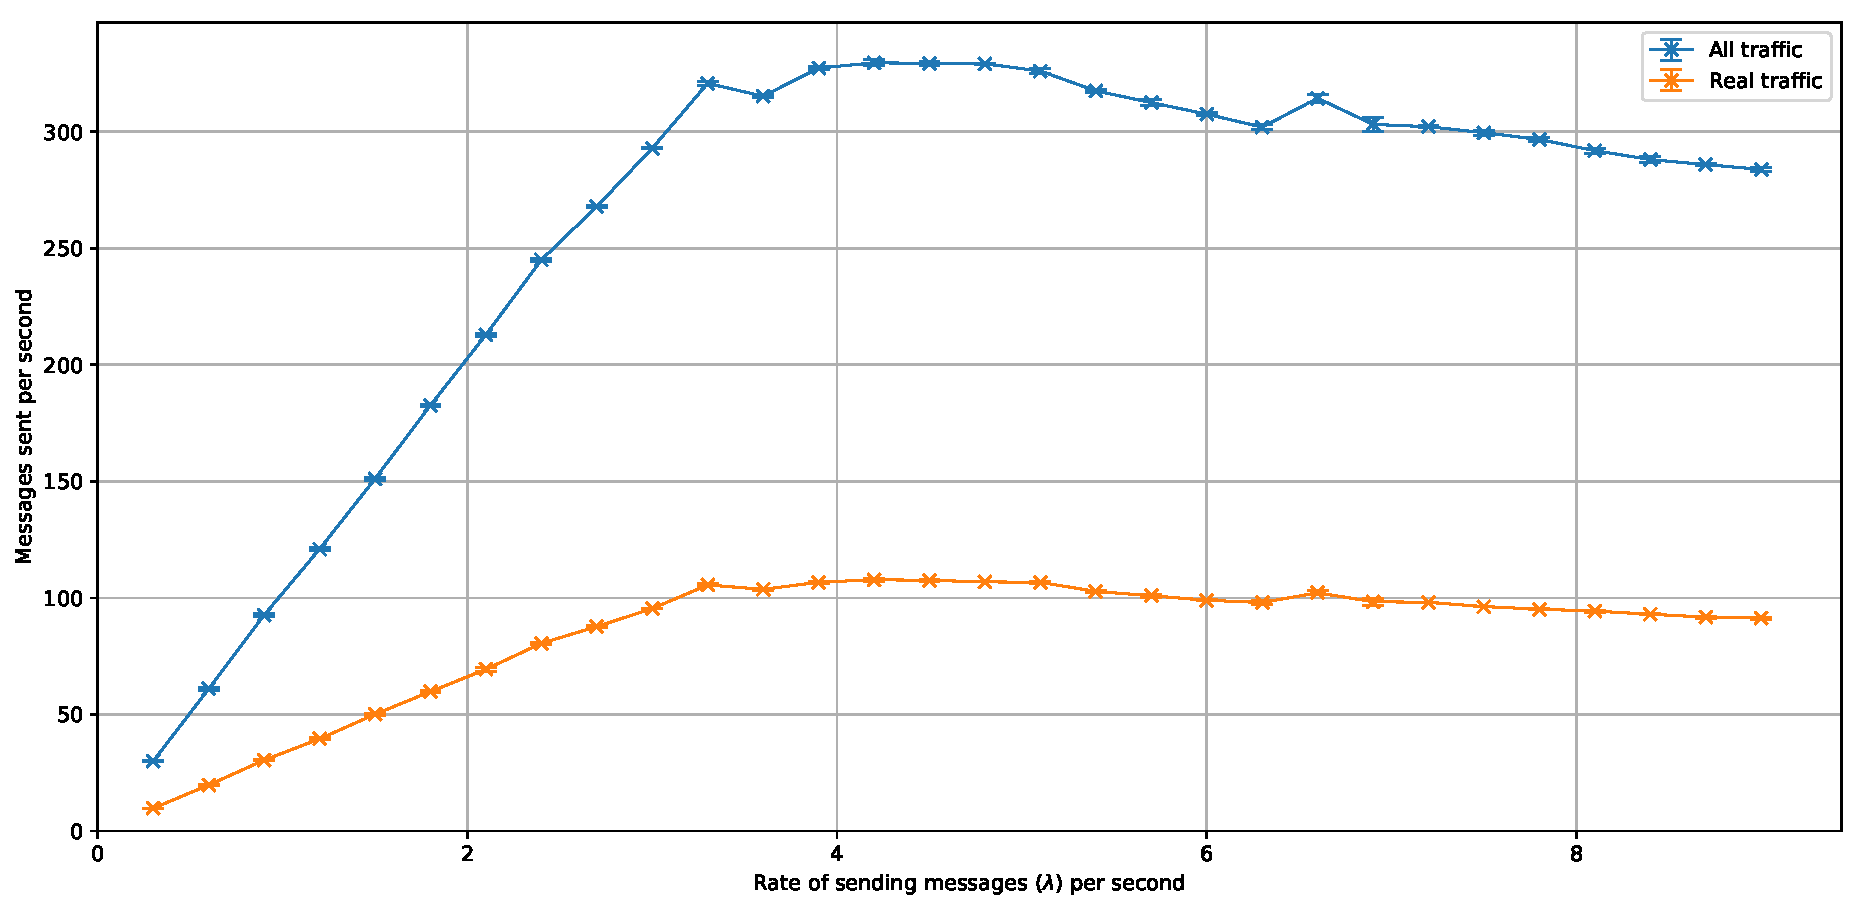
\includegraphics[width=\linewidth]{../figs/mix_bandwidth}
	\caption{Overall sent traffic and real traffic per second for a single mix node.}
	\label{fig:mix_bandwidth}
\end{figure}

Figure~\ref{fig:mix_bandwidth} shows the sending rate of all traffic and rate of real traffic versus the overall sending rate $\lambda$ of a client at a single Python mix node. Messages sent by the mix node includes forwarded messages and cover traffic generated by the mix node. Observe that the throughput of the mix node increases linearly until around the 325 messages per second mark. Beyond this point throughput stabilises before showing a small downward trend as the configured sending rate of a single client increases. This deviates from results demonstrated in the Loopix paper \cite{piotrowska2017loopix}, where throughput was linear until around the 225 messages per second mark, and a smaller growth was observed beyond that point instead of a downward trend.

\subsection{Latency}

Latency measurements were made by Java clients sending messages to themselves. Each message contains the timestamp at which the message was created. Messages are created when the client needs to send a real message to remove the delay between the transmission of real messages. The client then records the timestamp when it passes a decrypted payload to the application, after receiving and processing the message. Sending looped real messages was done to ensure that time synchronisation issues would not impact measurements. As the experiments were conducted on a single host, network latency is negligible.

A modification was made to the Python provider to add a new configuration parameter \verb|PUSH_MESSAGES|. When this option is set, providers will immediately forward messages to clients, instead of waiting for clients to send a \verb|PULL| request. This was necessary to measure end-to-end latency solely as a result of system overhead.

The latency experiments were configured with $\lambda_R = \lambda_D = \lambda_L = 2.67$ messages per second, and the per-hop delay is set to $0.0$ seconds. Values are measured by Java clients and averaged over 3 repetitions, and the error bars are the standard deviation.

\begin{figure}[h]
	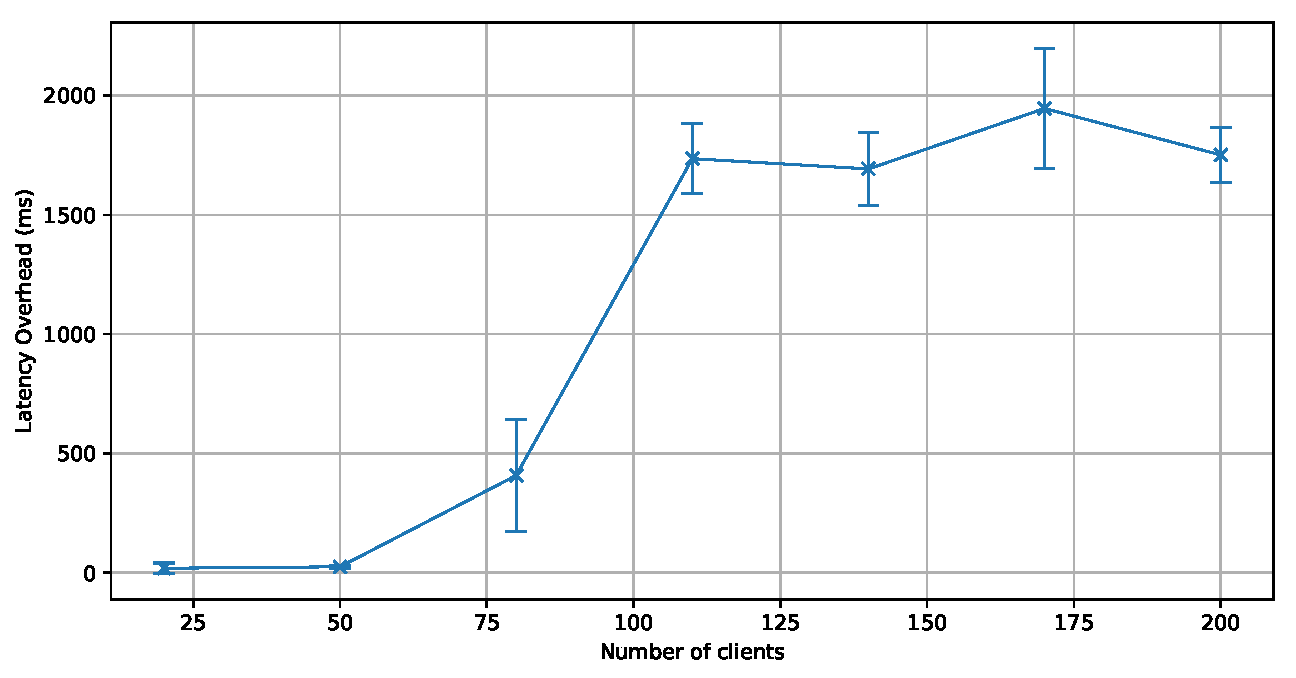
\includegraphics[width=\linewidth]{../figs/client_latency}
	\caption{Latency overhead measured as the time taken to send a message through the Loopix network, with increasing number of clients.}
	\label{fig:client_latency}
\end{figure}

The first experiment was conducted with \verb|PUSH_MESSAGES| enabled. The number of clients is varied from 20 to 200 clients, increasing by 30 each iteration. The type of clients are evenly split between Java and Python clients. The results are shown in Figure~\ref{fig:client_latency}. With 20 clients, the latency measured was \SI[separate-uncertainty=true]{19.08(2214)}{\milli\second}. This increases to \SI[separate-uncertainty=true]{25.22(672)}{\milli\second} with 50 clients. As the number of clients exceed 50, a bottleneck appears and the latency overhead exceeds \SI{1.5}{\second}. This bottleneck also manifests in the mix node bandwidth results in Figure~\ref{fig:mix_bandwidth}. 

My results differ significantly from the original paper \cite{piotrowska2017loopix}, where the end-to-end latency was measured at \SI{1.5}{\milli\second}. This discrepancy may be caused by my experiment's significantly higher rates of sending messages. The original paper uses $\lambda = 30\text{ messages per minute} = 0.5\text{ messages per second}$. 

\begin{figure}[h]
	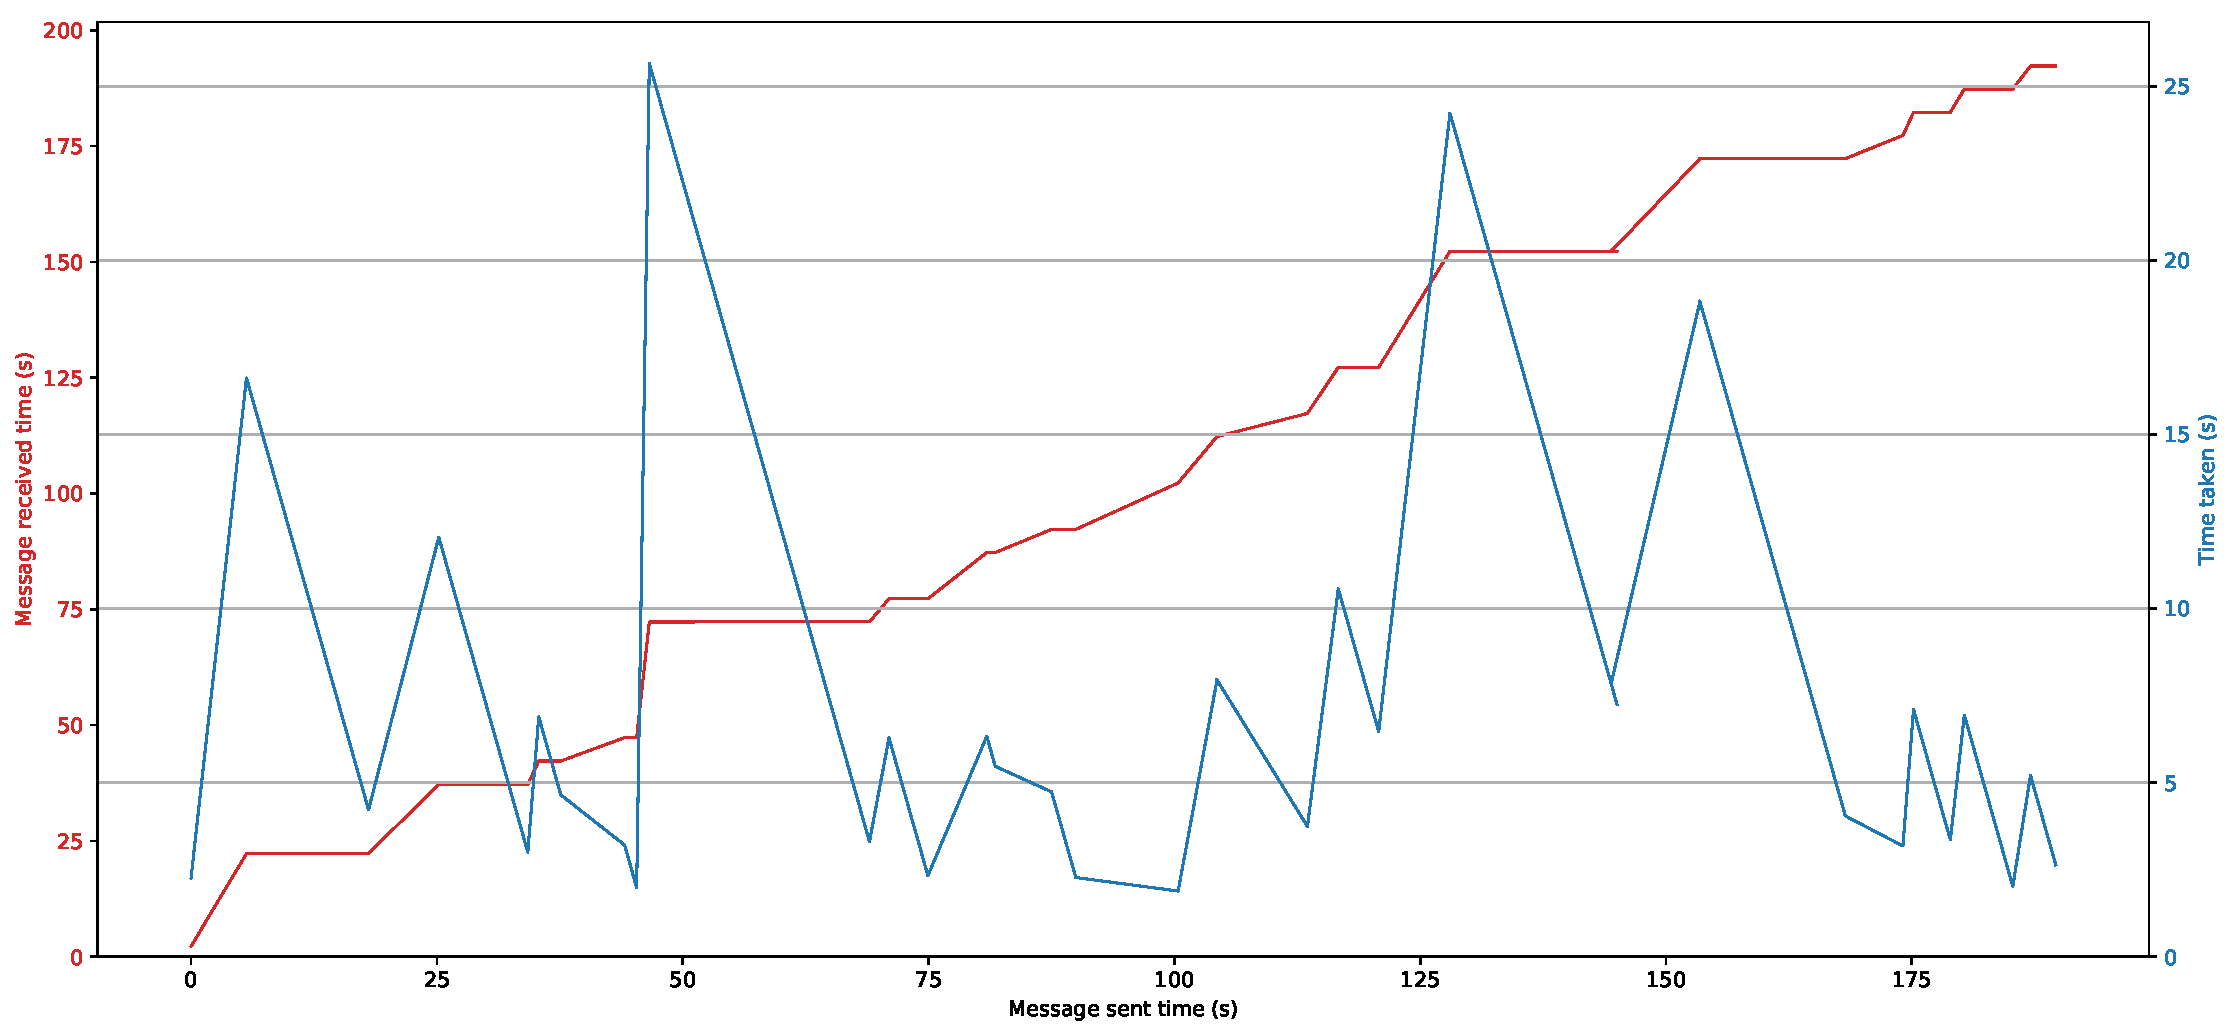
\includegraphics[width=\linewidth]{../figs/client_total_latency}
	\caption{Plot of message sent and received times, and the time taken over a 3 minute period.}
	\label{fig:client_total_latency}
\end{figure}

The next experiment disables \verb|PULL_MESSAGES|, and sets \verb|TIME_PULL| and \verb|MAX_RETRIEVE| such that the client will pull 30 messages every 5 seconds. The end-to-end latency measurement now includes time spent in the provider queue waiting for client requests.

Figure~\ref{fig:client_total_latency} plots the time a message is sent, the time the message is received, and the time taken taken to send and receive the message. Observe the periodic nature of the time taken plot, the result of periodically requesting messages from the provider. Ideally the longest time taken is around 5 seconds, which is the period between message retrieval by the client. However, this is not the case, likely due to a bottleneck somewhere in the system.

\section{Viability on Mobile Devices}

The key motivation for this project is to produce a library usable by mobile devices, specifically Android devices. Mobile devices are heavily resource constrained, especially with respect to cellular data usage and battery life. This section will explore the viability of Loopix on mobile devices in terms of energy use, data usage, and associated costs. The tuning of network parameters is also discussed.

\subsection{Bandwidth Usage}

Analysis of the bandwidth usage of a single Loopix client is straightforward. The network message send rates $\lambda_R, \lambda_L, \lambda_D$ yield an expected average send rate $\lambda_\text{send} = \lambda_R + \lambda_L + \lambda_D$, and \verb|TIME_PULL| and \verb|MAX_RETRIEVE| characterises the rate of incoming traffic $\lambda_\text{pull} = \texttt{MAX\_RETRIEVE}/\texttt{TIME\_PULL}$. As such, the total network traffic generated per second is $\lambda_\text{total} = \lambda_\text{send} + \lambda_\text{pull}$.

Suitable parameters need to be chosen first. A likely application of Loopix is for instant messaging. Assuming that for a usable experience, the total artificial delay ($4 * 1/\mu$) introduced should be below 1 second. Adding network latency of about \SI{200}{\milli\second} per hop with 4 hops and a message retrieval period of 1 second yields an end-to-end latency of about 3 seconds which is usable for instant messaging. Loopix's authors suggest that $\lambda/\mu \ge 2$ to maintain strong anonymity. Adding the delay constraint of $4* 1/\mu \le 1$, the following constraints are obtained: $\lambda \ge 2\mu, \mu \ge 4$. Using $\mu = 4, 1/\mu = 0.25\text{ seconds}$, $\lambda$ needs to be greater than 8 messages per second to maintain strong anonymity. $\lambda_\text{pull}$ needs to be greater than the rate of loop messages to ensure that the provider inbox can be emptied, else the inbox would continuously grow. $\lambda_\text{pull}$ is chosen to be $\lambda_\text{send}$ to allow at least a real message stream from a single client to be successfully retrieved.

Using the parameters described, $\lambda_\text{total} = \lambda_\text{send} + \lambda_\text{pull} = 8 + 8 = 16\text{ messages/second}$. At 2079 bytes per message, this yields $16\text{ messages/second} * \SI{2079}{\byte} = 33264\text{B}/\text{second} = \SI{2.68}{\gibi\byte}/\text{day} = \SI{80.3}{\gibi\byte}/\text{month}$. At \textsterling0.01 per MB, this would result in a monthly cost of \textsterling862.20, which is impractical.

It is possible to reduce the size of a message to $\sim1000$ bytes by reducing the size of the header by using IP addresses instead of host names, and reducing the size of packet body as well. However, reducing bandwidth use by half would still cost \textsterling431.10, which still is impractical. Without sacrificing anonymity, the delay added needs to be increased to bring $\lambda$ into reasonable values, however this would impact message responsiveness.

\subsection{Energy Usage}

To analyse energy use, EnergyBox \cite{vergara2014energybox} is used in conjunction with the packet traces captured for bandwidth analysis. EnergyBox was configured with energy models for a Nexus One connected to the TeliaSonera network. As the packet captures only contained 3 minutes of data, the output from EnergyBox was extrapolated to 24 hours. An assumption is made that because of the high message send rates, the radios and are never able to power down. This approach was verified by using a 3 hour packet trace with a send rate of 1.5 messages/second. This yielded \SI{6695}{\joule}, and extrapolating to 24 hours yields \SI{53562}{\joule}.

\begin{figure}[h]
	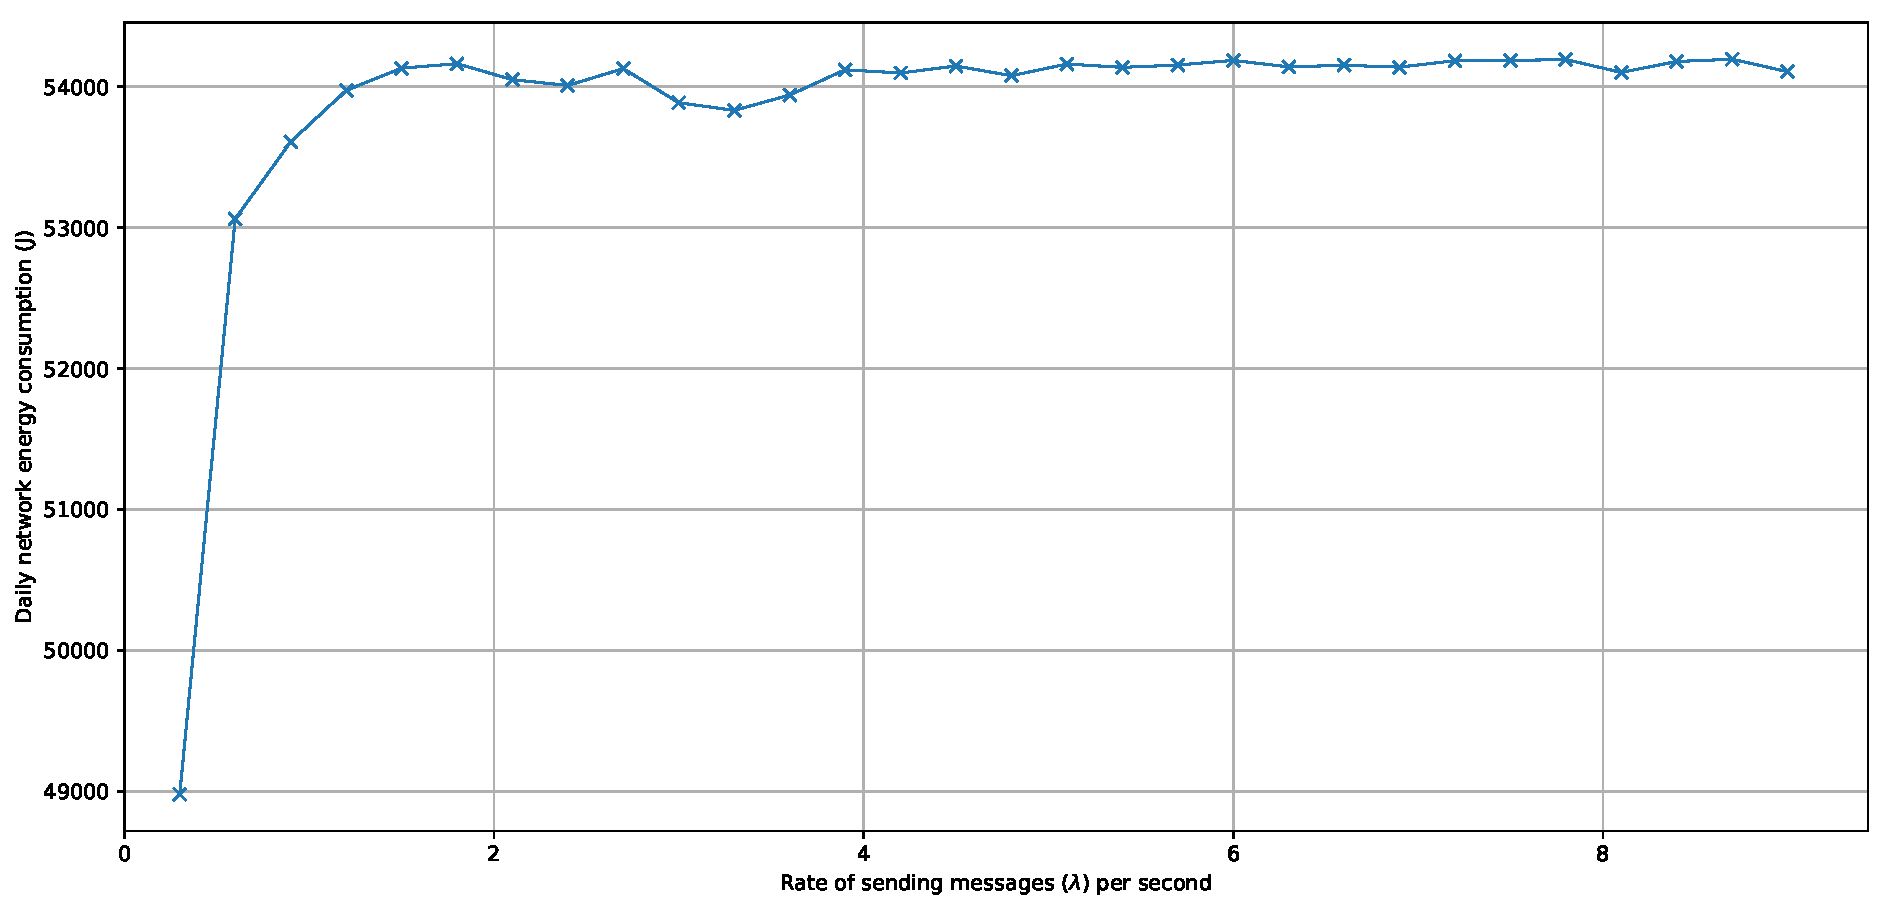
\includegraphics[width=\linewidth]{../figs/energy_use}
	\caption{Daily energy consumption of a Nexus One device connected to the TeliaSonera network with varying message send rates.}
	\label{fig:energy_use}
\end{figure}

In Figure~\ref{fig:energy_use}, observe that the daily energy consumption stabilises around the \SI{54000}{\joule} mark, or 15 Wh. A Nexus One has a battery capacity of 5.18 Wh. This means there is insufficient battery capacity to run Loopix for a whole day. Note that the energy consumption values accounts only for energy used for network communication, and does not include energy required to keep the device awake and generating Loopix messages.

As providers store messages for clients, it is possible to use a strategy of sending traffic only when the application is in the foreground, and perform periodic background polling for messages from the provider. This would reduce the bandwidth and energy used as the Loopix client would only be active for short bursts. However, the potential impact to anonymity is a concern, as this introduces traffic patterns which may leak information, but this is not explored.

\end{document}